\documentclass[12pt,a4paper]{article}
\usepackage[utf8]{inputenc}
\usepackage[german]{babel}
\usepackage[T1]{fontenc}
\usepackage{times}
\usepackage{graphicx}
\usepackage{url}
\usepackage[dvipsnames]{xcolor}
\usepackage{setspace}
\usepackage{enumerate}
\usepackage{pbox}
\usepackage{amsmath}
\usepackage{amsfonts}
\usepackage{amssymb}
\newcommand{\red}[1]{\textcolor{red} {#1}}
\newcommand{\blue}[1]{\textcolor{blue} {#1}}
\newcommand{\green}[1]{\textcolor{ForestGreen} {#1}}
\newcommand{\yellow}[1]{\textcolor{yellow} {#1}}
\newcommand{\nl}{\\[0.1cm]}
\newcommand{\ecb}[1]{\{#1\}}
\title{Algorithmic Game Theory}
\author{Henrik Tscherny}
\begin{document}
\maketitle
\tableofcontents



\section{Random Definitions}
\begin{itemize}
\setlength\itemsep{0.05cm}
\item \textbf{weakly solved}: outcome if both players play perfect
\item \textbf{strongly solved}: entire game tree/graph is known
\end{itemize}


\section{Non-Cooperative-Games}

Normalform $G = (P,S,u)$
\begin{itemize}
\item Players: $P = \ecb{1,2,...,n}$
\item Strategies: $S=(S_1, S_2, S_n)$
\item Utility functions: $u=(u_1,u_2,...,u_n)$ with $u_i: S \rightarrow \mathbb{R}$
\end{itemize}
Note: Only \textbf{one decision} is made (choice of strategy) and moves are \textbf{simultaneous}
Strategy Profile $s = (s_1,s_2,...s_n) \in S_1 \times S_2 \times ... \times S_n = S$
\\ 
\textbf{Weakly Dominant Strategies ($\leq$)}: The strategy has the best payoff regardless of the choices of the other players.
\\ 
\textbf{Strictly Dominant Strategies ($<$)}: The strategy has the greatest payoff among all other strategies. (there can only be at most one such strategy)


\subsection{pure and mixed strategies}
\textbf{pure strategies}:\\
every player chooses the same action in a given situation (like a spreadsheet on what to do). Each move is deterministic. Example: Play Paper every time in Rock-Paper-Scissors\\

\textbf{mixed strategies}:\\
use probabilities to determine a pure strategy for each situation. Each move is non-deterministic. Example: choose Rock, Paper, Scissors with p=1/3 each. \\
\begin{itemize}
\setlength\itemsep{0.05cm}
\item Models that players confuse each other by switching
\item adds uncertainty about actions of others
\item models repeated play and population dynamic
\end{itemize}


\subsection{Pareto}
\begin{itemize}
\setlength\itemsep{0.05cm}
\item \textbf{s weakly Parteo-dominates t}: $\forall i\in I: u_i(s) \geq u_i(t)$. \\
payoff of s is at least as good as for t for each utility function
\item \textbf{s Pareto-dominates t}: $\exists j \in I: u_j(s) > u_j(t)$.\\
payoff of s is better than for t for a given utility function\\
\item \textbf{s strongly Pareto-dominates t}: $\forall i \in I: u_i(s) > u_i(t)$.\\
payof of s is better than for t for all utility functions
\item \textbf{t is Pareto-optimal}: $\neg \exists s\in S: \text{ s Pareto-dominates t}$\\
\item \textbf{t is weakly Pareto-optimal}: $\neg \exists s\in S: \text{ s stongly Pareto-dominates t}$
\end{itemize}

In a Pareto optimum no Player can gain switch strategies without another player being worse off
\\
\textbf{Example}: (S, S), (S, C), (C, S) are Pareto-optimas for the prisoners dilemma.\\
(S, S) strongly dominates (C, C).\\
All strategies in rock paper scissors are pareto-optimal
\\
\textbf{Best Response}: A Strategy is a best response to another strategy iff it produces the best payoff for the player given the strategies of the other players
\\
Note: dominant strategy $\rightarrow$ best response but not $\leftarrow$


\subsection{Nash}

\textbf{pure}:\\
\begin{itemize}
\setlength\itemsep{0.05cm}
\item \textbf{Nash equilibrium in pure strategies}: $\forall i \in I: s_i \text{ is a best response to } s_{-1}$
\item \textbf{strict Nash equilibrium in pure strategies}: $\exists ! s: s \text{ is a best response to } s_{-1}$\\
$s_{-i}$ is the strategy profile s without the strategy of player i
\end{itemize}
The prisoners dilemma has (C,C) as the single pure Nash equilibrium where every player plays his dominant strategies.\\
There can be none, one or multiple such equilibria\\
Note: The pure Nash equilibria can be computed in \textbf{PTIME} by exhaustive search for best response\\
\subsubsection{Nashs Theorem}
For a non-cooperative game G with finite Players, finite Strategies there exists a Nash equilibrium in mixed strategies\\
\textbf{Proof sketch}:
\begin{itemize}
\setlength\itemsep{0.05cm}
\item Model strategies as unit vectors in $\mathbb{R}^{|S|}$
\item Mixed strategies are points on a simplex in this vector space
\item define some function $f : \Pi \rightarrow \Pi$ ($\Pi$ is the set of all mixed strategy profiles)
\item use Brouwers fixpoint theorem to show that f has at least one fixpoint
\end{itemize}
\subsubsection{Computation}
\begin{itemize}
\item translate problem intro mixed integer programming
\item solve MIP (NP-complete)
\item Given a Nash equilibrium for a game, finding the next equilibrium is FNP-compete
\begin{itemize}
\item Functional Complexity: Functions that given input x can be compute some y in some Time/Space
\item FP and FNP are functional P and NP
\end{itemize}
\end{itemize}


\subsection{Prisoners Dilemma}
\begin{itemize}
\setlength\itemsep{0.05cm}
\item $P = \ecb{1,2}$
\item $S_1 = S_2 = \ecb{S,C}$
\item $S = \ecb{(S,S),(S,C),(C,S),(C,C)}$
\item $u_1 = \ecb{(S,S)\mapsto 4, (S,C) \mapsto 0, (C,S) \mapsto 5, (C,C) \mapsto 3}$ 
\item $u_2 = \ecb{(S,S)\mapsto 4, (S,C) \mapsto 5, (C,S) \mapsto 0, (C,C) \mapsto 3}$ 
\end{itemize}

\section{Sequential Games}
\begin{itemize}
\setlength\itemsep{0.05cm}
\item Several decisions
\item Strategies can be seen as advice
\item Players move sequentially
\item can be represented using a Graph (maybe even Tree) (e.g. in Chess board state diagram)
\end{itemize}
\textbf{Complete Information}: All players know possible moves and utilities of all players\\

\subsection{Zermelos Theorem}
Every finite sequential game tree has a solution (strategy profile and utility) that can be obtained by backward induction\\
\textbf{Backwards Induction}
\begin{itemize}
\setlength\itemsep{0.05cm}
\item start at the last round of the game (only one decision is left)
\item determine for each of those nodes (in this depth) the best choice for the current player (and delete the rest)
\item move one layer up and repeat till you reach root (only one path is left)
\end{itemize}


\section{Combinatorial Games}
Can be solved using backwards induction
\begin{itemize}
\setlength\itemsep{0.05cm}
\item Two Players
\item Either One Player wins (1) and the other loses (-1) or its a draw (0)
\item zero-sum-game
\end{itemize}

\textbf{Geography is PSPace-complete}
\begin{itemize}
\item $\in PSapce$: use DFS on game tree and only keep current path in memory (depth is poly)
\item $hardness$: by reduction to TrueQBF:
\begin{itemize}
\item $\varphi = \exists p_1 \forall p_2\cdots . \psi$ with $\psi = \psi_1 \land \cdots \land \psi_m$
\item 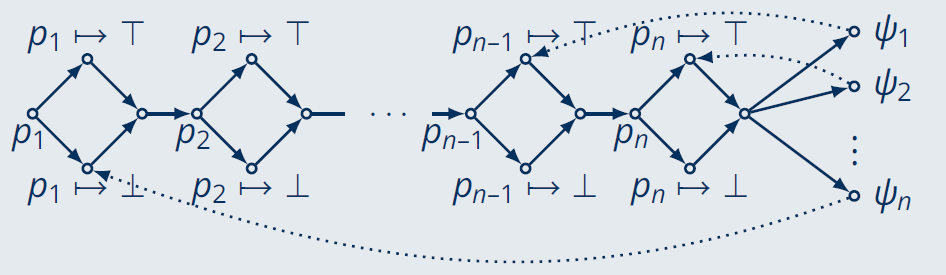
\includegraphics[scale=0.4]{./resources/geo.png}
\item 'diamonds' select for each prop-var if its true/false and in the end formula gets checked by edges to diamond nodes
\item Example:\\ 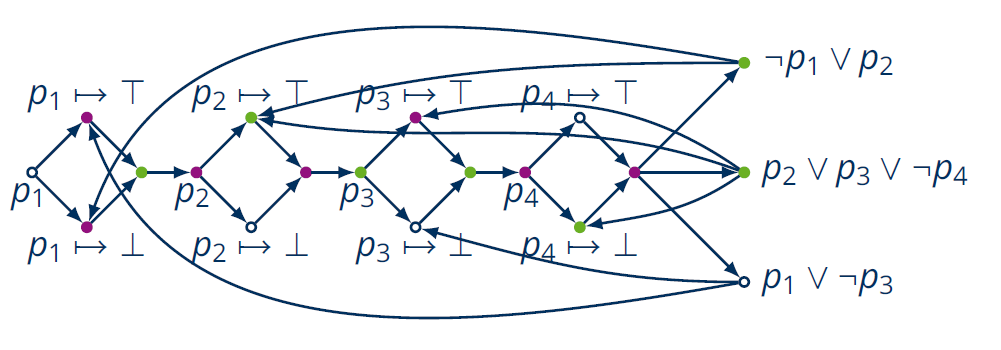
\includegraphics[scale=0.4]{./resources/geoEx.png}
\end{itemize}
\end{itemize}

\section{Minimax Tree Search}
used to solve zero-sum games
\begin{itemize}
\setlength\itemsep{0.05cm}
\item there is a min and a max player 
\item if min players turn select child node with min value (analogous for max)
\item min and max switch in each layer 
\item Complexity: $O(b^d)$ (b: branching factor, d: depth), hence its impractical for larger games
\item $\rightarrow$ solution: alpha beta pruning:
\begin{itemize}
\item stop search when when we know that a nodes does not gets visited anyway
\item Example: \\ 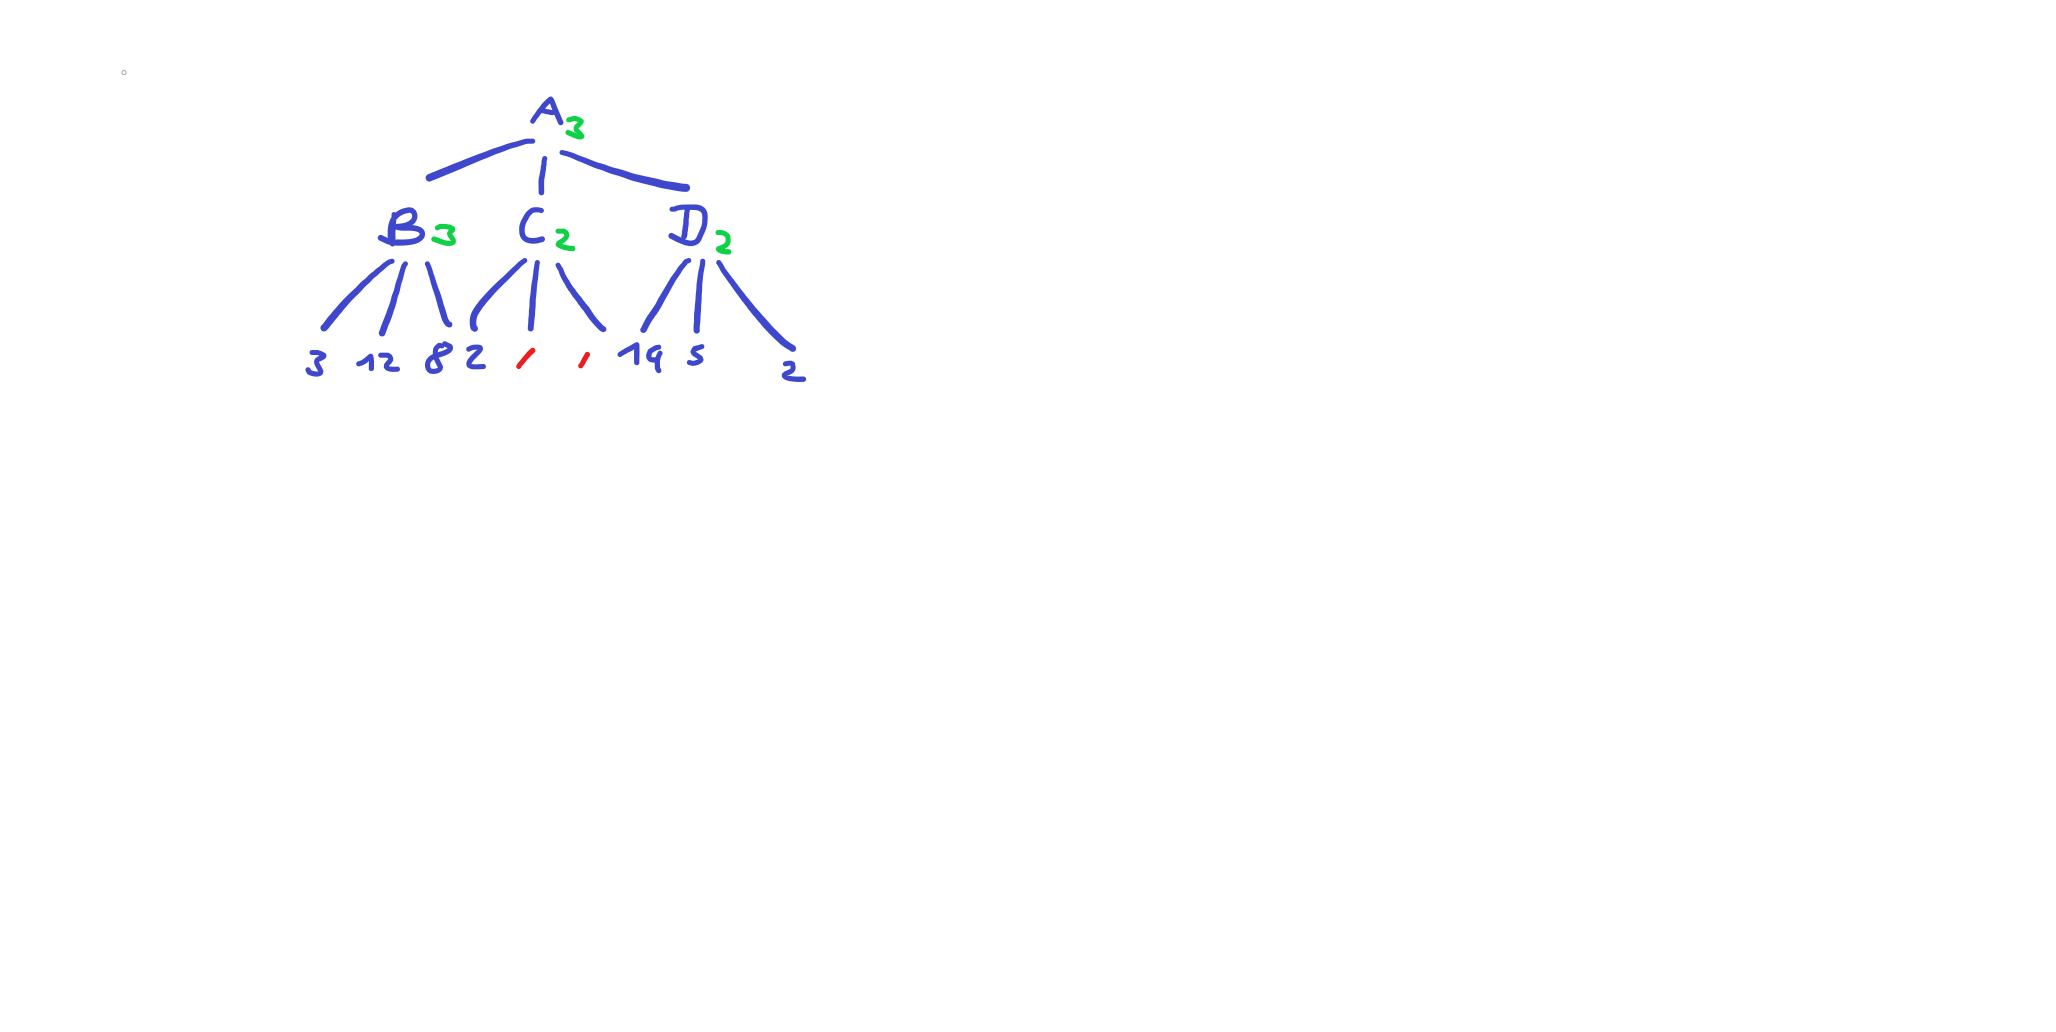
\includegraphics[scale=0.4]{./resources/ab_search.png}
\item because B is already 3 we can stop at C=2 because Max does not care anyway
\item we have to search all of D because D=2 is the right most element (unlucky) 
\item better heuristic helps
\item Worst-case complexity: $O(b^d)$ (all nodes have to be searched (because they are on the right))
\item Best-case complexity: $O(\sqrt{b}^d)$ (left nodes terminates search already)
\end{itemize}
\end{itemize}

\end{document}
